\begin{center}

  \begin{tabular}{rp{16cm}lp{20cm}}%{rl}

  % after \\: \hline or \cline{col1-col2} \cline{col3-col4} ...

  论文地址:& \href{https://arxiv.org/abs/1511.05644}{https://arxiv.org/abs/1511.05644} \\
  来源:& ICLR, 2016 \\
  作者:& Alireza Makhzani ,Jonathon Shlens ,Navdeep Jaitly ,Ian Goodfellow ,Brendan Frey \\
  源码:& \href{https://github.com/fducau/AAE_pytorch}{AAE\_pytorch} \\

%  slides:& \href{http://yunshengb.com/wp-content/uploads/2017/03/nips_2018_r2l_workshop_talk.pdf}{{\footnotesize Convolutional Set Matching for Graph Similarity}}\\

  关键词:& \textbf{GAN, Autoencoder, Generative Models} \\

  写于:& \date{2020-12-20}

  \end{tabular}

\end{center}

论文\cite{makhzani2016adversarial}对autoencoder进行了改进,结合GAN提出了新的generative model。第一次看了一两页,看的很懵,第二次看的时候十分痛快,一个上午就看完了,整篇论文读下来收获很多。Adversarial Autoencoder(AAE)将GAN与autoencoder相结合,仿照GAN的训练方式来训练自编码器网络。通篇看下来,autoencoder、GAN、AAE都成了分布的匹配(拟合)问题。特别是论文提出的AAE,论文将数据分布$p_d(\boldsymbol{x})$的隐变量$\boldsymbol{x}$的分布与某个已知的分布进行匹配/拟合。论文中不仅给出了基础的AAE的架构,如图Fig.\ref{fig:AAE}所示,还给出了AAE在其他方面的应用,如有/无/半监督的AAE、AAE在聚类和降维上的应用,并给出了相应的网络结构,非常棒!

\begin{figure}[h]
	\centering
	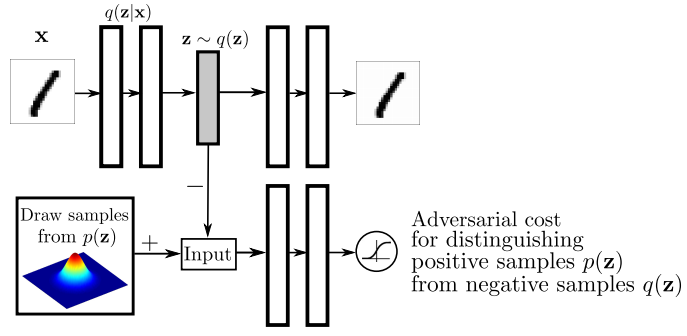
\includegraphics[width=.8\textwidth]{pics/aae.PNG}
	\caption{Architecture of AAE}
	\label{fig:AAE}
\end{figure}

\paragraph{AAE思路}
通常的autoencoder或者VAE\cite{kingma2014autoencoding}在训练时通常是以重建损失或者ELBO为目标,VAE中使用了重参数化的技巧来训练。AAE其实和VAE也是有一点相似之处的:都会从一个确定的分布中进行采样。对AAE而言,整个网络结构分为两部分:autoencoder和discriminator。autoencoder就是普通的自编码器:输入数据学习到数据的隐表示$\boldsymbol{z}$,使用重建损失函数;discriminator与GAN中的D时一致的:从一个已知的先验分布$p(\boldsymbol{z})$中采样一个$\boldsymbol{z}$,这个时候来自autoencoder的$\boldsymbol{z}$作为负样本$\boldsymbol{z}_-$,来自$p(\boldsymbol{z})$作为正样本$\boldsymbol{z}_+$,由D来进行判别,使用判别损失函数。如果与GAN进行比较,可以知道\tbc{red}{$p(\boldsymbol{z})$相当于真是数据分布,而autoencoder中的encoder则相当于GAN中的generator}。上文中还提到了一个很关键的点:\tbc{red}{分布的匹配/拟合}。

这在AAE中体现的尤为明显。上面描述的过程其实也可以抽象为分布的匹配/拟合。已知的分布$p(\boldsymbol{z})$作为一个目标分布,目的是使数据隐变量的分布$p(\boldsymbol{z})$与目的分布一致 --- 判别器无法区分$\boldsymbol{z}$是来自$p(\boldsymbol{z})$还是来自$q(\boldsymbol{z})$。与VAE中的重参数化不同,AAE可以直接使用梯度下降的方法进行训练。AAE的训练过程分为两个阶段:reconstruction和regularization。

在reconstruction阶段:autoencoder通过最小化重建损失来更新encoder和decoder。在regularization阶段:通过对抗损失来更新判别网络和生成网络(也即encoder)。



\paragraph{AAE的应用}
论文中还介绍了AAE的几个主要的应用:
\begin{itemize}
	\item 将标签信息融入到判别器中:以one-hot的形式构造标签编码,将标签编码与从$p(\boldsymbol{z})$中采样到的$\boldsymbol{z}$一起输入到判别网络中
	\item 将标签信息融入到autoencoder中:将one-hot编码的标签信息与数据的隐变量$\boldsymbol{z}$一起输入到decoder中
	\item 半监督的AAE:其实这个相当于将标签信息融入到autoencoder和判别器中。此时的网络结构中将会由两个判别器,分别对$\boldsymbol{z}$和标签信息进行判别,因此也需要为标签信息增加一个generator --- 论文中采用的是categorical分布。此时网络的训练在原基础上增加了一个阶段 --- semi-supervised classification阶段,该阶段使用交叉熵来更新监督损失
	\item 使用AAE进行无监督的聚类:这部分十分有趣!论文中特地针对MINST数据集进行了聚类,但不是聚类成10类,AAE可以将同一个数字的不同风格的图像区分出来 --- 将风格分离了出来
	\item 使用AAE进行降维:此处的AAE与半监督的AAE十分相似。论文中还分析了已有方法进行降维时的几个主要问题:难以应用到新的数据上(T\_SNE解决了这个问题)、数据可能处于流形空间等
\end{itemize}

\paragraph{方法解决的问题/优势}
\begin{itemize}
	\item 将GAN中的discriminator与autoencoder相结合,得到了强大的自编码器
	\item 不需要使用重参数化就能训练,效果比VAE好
	\item AAE的结构修改可以使用到多种任务上,可扩展性极好
\end{itemize}

\paragraph{方法的局限性/未来方向}
\begin{itemize}
	\item 用来学习更好的表征,很棒的特征提取器
	\item \tbc{red}{基于AAE的聚类}
	\item \tbc{red}{基于AAE的降维可视化}
\end{itemize}